% ============================================================
% Drop-in section to replace the placeholder
%   "Pls show a case, e.g. bandit related to the definition..."
% Macros used (already in main.tex preamble):
%   \Rmax \PiK \Vhi \Vlow \Rex \Dstruct \ModE \Ex
% Labels referenced (from the Results sections in backup.tex):
%   def:exreg, def:sound, prop:nothing, lem:bridge, thm:nofree
% Figure: examiner_bandit_demo.pdf  (three panels A/B/C)
% ============================================================

\section{A Worked Case: The Examiner in a Bandit}
\label{sec:bandit}

The simplest world in which our definitions become concrete has no state at all.
A multi-armed bandit is our stream with $|\mathcal{S}|=1$ and $H=1$, and we use it for
two reasons: it is the standard sanity check for any value-based definition, and it
makes the two gaps of Theorem~\ref{thm:nofree} maximally transparent, since
``a behaviour the learner never tried'' becomes simply ``an arm it never pulled.''

\paragraph{Setting.} There are $N$ arms; pulling arm $i$ returns a reward
$r\in\{0,1\}$ with unknown mean $\mu_i$, so $\Rmax=1$. All arms pay $\tfrac12$ except a
single \emph{special} arm with $\mu_{i^\star}=\tfrac12+\epsilon$, and the agent acts on
one never-resetting stream. Write $\hat\mu_i$ for the empirical mean of arm $i$, $n_i$
for its pull count, and $c_i=\sqrt{2\ln t / n_i}$ for the confidence half-width, with
$c_i$ at its maximum for an arm that has never been pulled.

\paragraph{The definitions become arithmetic.} With $H=1$ the value of the policy
``pull arm $i$'' (Definition~\ref{def:basic}) is just the arm mean,
$f^{\pi}_t=\mu_i$. If every arm is representable, the within-capacity optimum
(Definition~\ref{def:capcomp}) is $f^{K_L}_t=\mu^\star=\tfrac12+\epsilon$ and the
structural gap vanishes, $\Dstruct_t=0$. The learner $\mathcal{L}$ is the rule that
selects the played arm $a_t$; the examiner $\mathcal{E}$ (Definition~\ref{def:agent})
reads its two numbers off the same counters,
\[
\Vhi=\max_i\big(\hat\mu_i+c_i\big),
\qquad
\Vlow=\hat\mu_{a_t}-c_{a_t},
\]
an optimistic ceiling over \emph{all} arms and a pessimistic floor on the
\emph{played} arm. Its inductive bias $\ModE$ is exactly the concentration assumption
that lets $c_i$ shrink with data. The examiner regret (Definition~\ref{def:exreg}) is
then the confidence width,
\[
\rho_t=\Vhi-\Vlow=\max_i\big(\hat\mu_i+c_i\big)-\big(\hat\mu_{a_t}-c_{a_t}\big),
\]
which depends only on counts and empirical means, never on $\mu$ or $\mu^\star$.
These are not new objects: $\sum_t (f^{K_L}_t-f^{\pi_t}_t)=\sum_t(\mu^\star-\mu_{a_t})$
is the classical pseudo-regret, and $\sum_t\rho_t=O(\sqrt{NT\log T})$ is the standard
UCB confidence-width sum \citep{auer2002ucb,lai1985asymptotically}. \textbf{[cited]}

\paragraph{Soundness, and where honesty lives.} By Hoeffding's inequality both
soundness conditions of Definition~\ref{def:sound} hold with high probability: the
floor is real, $\hat\mu_{a_t}-c_{a_t}\le\mu_{a_t}$, and the ceiling is real,
$\max_i(\hat\mu_i+c_i)\ge\mu^\star$, with slack $\delta_t$ equal to the Hoeffding
failure margin, which vanishes as counts grow. The mechanism is one line: an arm that
has \emph{never} been pulled keeps $c_i$ at maximum, so its optimistic index stays
high and the ceiling $\Vhi$ cannot fall. The examiner is structurally forbidden from
reporting ``no room to improve'' about an arm it has not inspected; a dishonest
examiner is precisely one that discards this and assumes the unseen arm is ordinary.

\paragraph{The three results, instantiated (Figure~\ref{fig:bandit}).}
Proposition~\ref{prop:nothing} appears when the trivial examiner reports
$\rho_t\equiv0$ for both a good (UCB) and a bad (fixed-arm) learner: identical
self-reports, while true regret levels off for one and grows linearly for the other
(panel~A). Lemma~\ref{lem:bridge} appears in a coverable world ($N=5$), where the
sound certificate $\sum_t\rho_t$ stays above the true regret throughout, a valid if
loose ceiling on what remains removable (panel~B). Theorem~\ref{thm:nofree} appears
once the world outruns the horizon ($N>T$) and the special arm is placed out of
reach: the sound examiner honestly keeps $\rho_t$ large, signalling uncovered ground,
while a biased examiner that assumes a shared mean collapses $\rho_t$ toward zero and
reports a false ``done'' even as true regret climbs at rate $\epsilon$ (panel~C).

\begin{figure}[t]
\centering
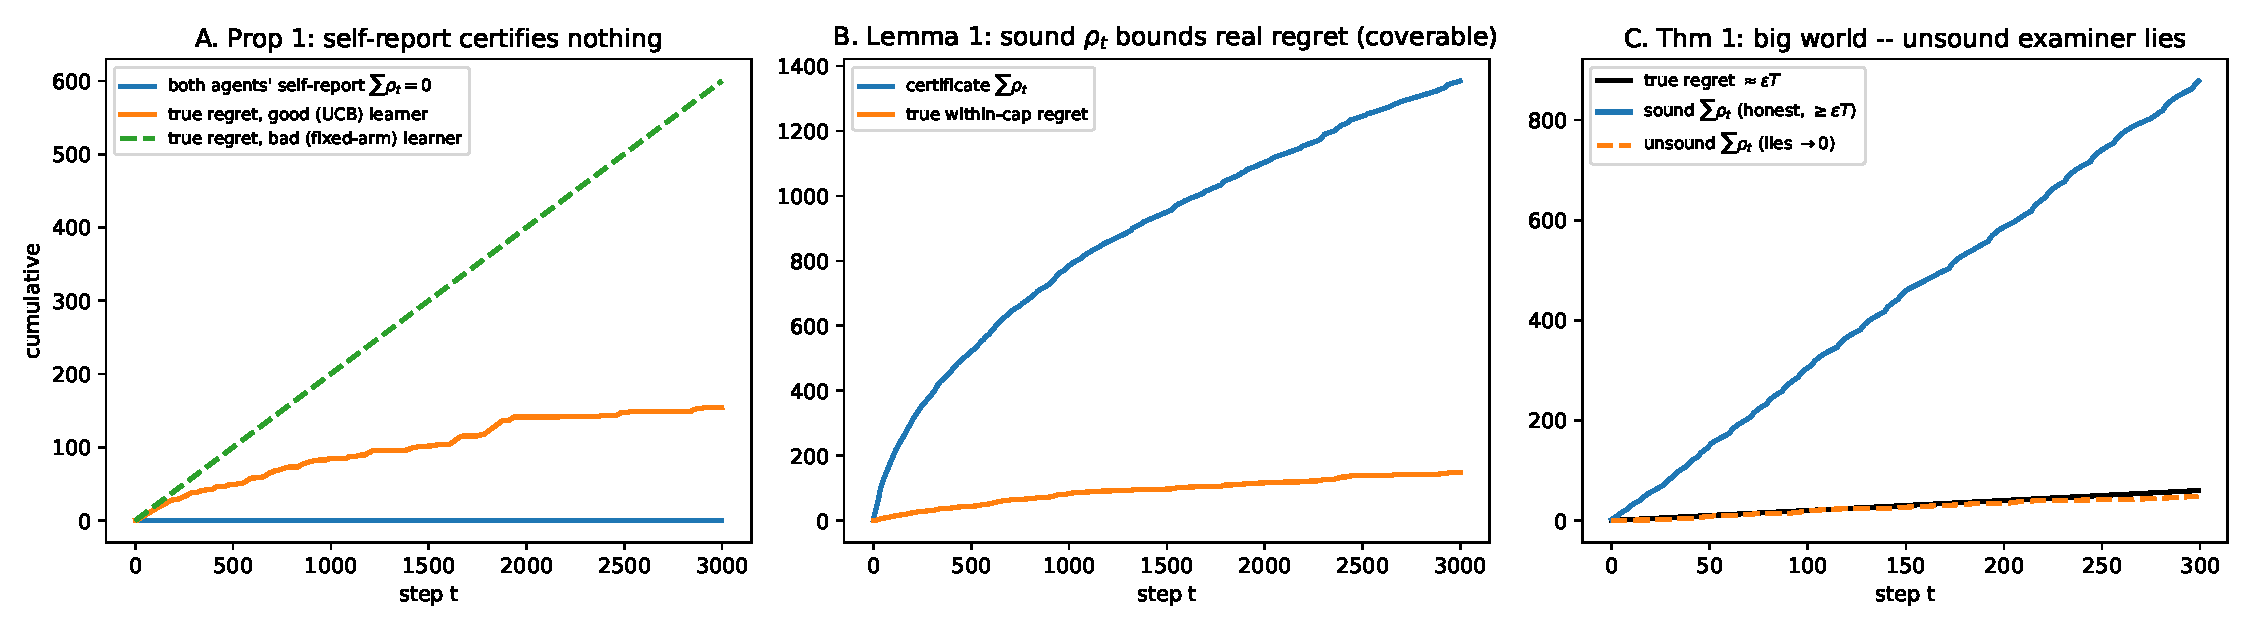
\includegraphics[width=\textwidth]{examiner_bandit_demo.pdf}
\caption{The examiner in a bandit. \textbf{(A)} Proposition~\ref{prop:nothing}: two
agents with the identical self-report $\sum_t\rho_t=0$ differ arbitrarily in true
regret. \textbf{(B)} Lemma~\ref{lem:bridge}: in a coverable world the sound
certificate $\sum_t\rho_t$ upper-bounds the true within-capacity regret. \textbf{(C)}
Theorem~\ref{thm:nofree}: when the world outruns the horizon, a sound examiner keeps
$\rho_t$ large (honest), while a biased examiner drives $\rho_t$ below the true regret
(unearned confidence).}
\label{fig:bandit}
\end{figure}

\paragraph{How to use it.} The bandit shows the three intended uses without any
external optimum. As a \emph{monitor}, $\rho_t$ is an online read of self-assessed
room to improve; as a \emph{comparison metric}, two algorithms on one stream are
ranked by which $\rho_t$ shrinks faster toward its capacity-constrained optimum; and
as an \emph{audit}, a low $\rho_t$ is trustworthy exactly on the covered region, with
Theorem~\ref{thm:nofree} marking when no audit is possible and apparent convergence
should instead trigger exploration or external testing.
